\newpage
\section*{Objetivos}
En base a la planilla de requerimientos suministrada, sintetizar un circuito basado en amplificadores operacionales que satisfaga esos requisitos.

\section*{Metodología}
En general, para cada uno de los casos particulares solicitados se debe:
\begin{enumerate}
    \item Realizar una sintética introducción teórica.
    \item Analizar el circuito propuesto, su desarrollo numérico y todos los cálculos analíticos.
    \item Realizar simulación en LTSPICE.
    \item Armar el circuito y hacer las mediciones en laboratorio.
    \item Finalmente, comparar los valores calculados, simulados y medidos, y extraer conclusiones acerca de las diferencias. Analizar las causas.
    \item Presentar un informe digital y en papel.
\end{enumerate}

\section*{Desarrollo}

\subsection*{Circuito I}
En base a la planilla de requerimientos de la figura 1 se pide:
\begin{enumerate}
    \item Aproximar la función de atenuación mediante polinomios de Chebychev utilizando Python o MATLAB (ver Anexo I y II).
    \item Sintetizar un circuito que satisfaga los requerimientos del punto anterior utilizando topologías bicuadráticas de realimentación positiva o negativa a elección.
    \item Simular cada etapa y el filtro total con LTSPICE.
    \item Calcular la sensibilidad de la frecuencia del polo de cada bicuadrática (\(\omega_p\)) y del ancho de banda (\(\omega_p / Q_p\)).
    \item Analizar la peor desviación si todos los elementos tienen una tolerancia del 10\%.
    \item Realizar una simulación de Montecarlo de las desviaciones con LTSPICE.
    \item Armar el circuito, medir experimentalmente las curvas de atenuación y desfasaje. Contrastarlas con las predicciones teóricas y las simulaciones.
\end{enumerate}

\begin{figure}[H]
    \centering
    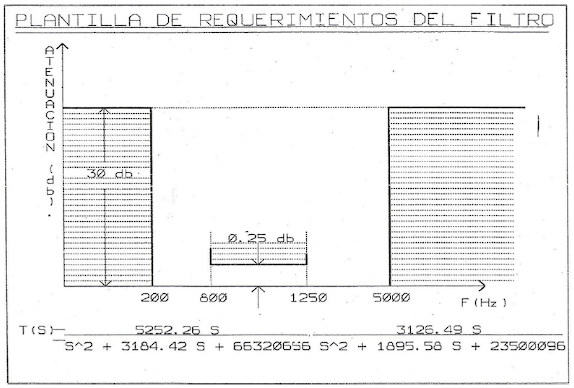
\includegraphics[width=1\linewidth]{figuras/imagen 1.PNG}
    \caption{Planilla de requerimientos}
\end{figure}
